% All Rights Reserved @apsitdevopsclub
% Information Technology Department
% A.P.Shah Institute of Technology, Thane
\documentclass[12pt,oneside,a4paper]{report}

\usepackage{amsmath}
\usepackage{amsfonts}
\usepackage{amssymb}
\usepackage{fullpage}
\usepackage{graphicx}
\usepackage{float}
\usepackage{textcomp}
\usepackage{pdfpages}
\usepackage{graphicx}
\usepackage{caption}
\usepackage{tikz} % Border ke liye zaroori package


\textwidth 6.5in
\textheight 9.5in
\bibliographystyle{plain}
\renewcommand{\bibname}{References}

\begin{document}

% --- FRONT MATTER (bina page numbers ke) ---
\pagestyle{empty} % Is section ke sabhi pages ke liye page number hide karega

% Ensure \usepackage{tikz} is in your main .tex file's preamble.
\begin{titlepage}

\begin{tikzpicture}[remember picture, overlay]
    \draw[line width=1.5pt]
        ([xshift=1.5cm, yshift=-1.5cm]current page.north west)
        rectangle
        ([xshift=-1.5cm, yshift=1.5cm]current page.south east);
\end{tikzpicture}

\vspace*{0.20cm}
{\centering
A Project Report on\\
\vspace{0.5cm}
{\Large\textbf {InferX-ML: 
Automated ML Pipeline for Training and Inference
}}\\
\vspace{0.5cm}
 Submitted in partial fulfillment of the requirements for the award\\
of the degree of\\ \vspace{1cm}
{\large\textbf {Third Year Engineering}}\\
\vspace{0.3cm}
in \\
\vspace{0.3cm}
{\large\textbf {Information Technology}}\\
\vspace{0.5cm}
by\\
\vspace{0.5cm}

\begin{tabular}{l l}
{\large \textbf{Bharatkumar Gungoman}} & {\large \textbf{(23104087)}} \\
{\large \textbf{Alok Gupta}}            & {\large \textbf{(23104045)}} \\
{\large \textbf{Om Babar}}   & {\large \textbf{(23104217)}} \\
\end{tabular}

\vspace{1cm}

Under the Guidance of\\ 
\vspace{0.3cm}

\hspace{.05cm} {\large \textbf {Ms. Sneha Dalvi }}\\
%\hspace{.05cm} {\large \textbf {Name of Co-Guide }}\\ 
\vspace{1cm}
\begin{figure}[h]
\centering

\includegraphics[scale=0.30]{apsit_logo.jpg}
\end{figure}

\hspace{.04cm}
\hspace{.04cm}

{\textbf {Department of Information Technology}}\\
\textbf{\textsf{NBA Accredited}}\\
A.P. Shah Institute of Technology\\
G.B.Road,Kasarvadavli, Thane(W)-400615\\
UNIVERSITY OF MUMBAI\\
\vspace{0.2cm}
\textbf{Academic Year 2025-2026}\\
}
\end{titlepage}
\clearpage


\newpage
\begin{tikzpicture}[remember picture, overlay]
    \draw[line width=1.5pt]
        ([xshift=1.5cm, yshift=-1.5cm]current page.north west)
        rectangle
        ([xshift=-1.5cm, yshift=1.5cm]current page.south east);
\end{tikzpicture}

\thispagestyle{empty}
\begin{center}
 \large\textbf{CERTIFICATE}
\end{center}
\vspace{1cm}

\par This to certify that the Mini Project-2B report on \textbf{``InferX-ML: Automated ML Pipeline for Training and Inference''} has been submitted by \textbf{``Bharatkumar Gungoman'' (23104087)}, \textbf{``Alok Gupta'' (23104045)}, and \textbf{``Om Babar'' (23104217)} who are bonafide students of A. P. Shah Institute of Technology, Thane as a partial fulfillment of the requirement for the degree in \textbf{Information Technology} during the second half of academic year \textbf{2025-26}, in the satisfactory manner as per the curriculum laid down by University of Mumbai.

\vspace{25mm}
%\hfill
\begin{tabular}{@{}l@{}}
Ms Sneha Dalvi\hspace{69mm}       Dr. Kiran Deshpande\\
Guide \hspace{94mm}      HOD, Information Technology\\

%\vspace{5mm}\\
\end{tabular}
\vspace{30mm}\\
\hfill
\begin{tabular}{@{}l@{}}

\vspace{5mm}
\end{tabular}


\vspace{15mm}
External Examiner\hspace{60mm}       Internal Examiner\\
\\1. \vspace{10mm} \hspace{90mm}       1.\\
\\

\vspace{1mm}
Place:A.P.Shah Institute of Technology, Thane\par
\vspace{1mm}

Date:
\clearpage

\vspace{5mm}


\clearpage

\newpage
\begin{tikzpicture}[remember picture, overlay]
    \draw[line width=1.5pt]
        ([xshift=1.5cm, yshift=-1.5cm]current page.north west)
        rectangle
        ([xshift=-1.5cm, yshift=1.5cm]current page.south east);
\end{tikzpicture}
\thispagestyle{empty}

\vspace*{-1cm} 

\begin{center}
    \large\textbf{Acknowledgement}
\end{center}

\vspace{1cm} 

\par
This project would not have come to fruition without the invaluable help of our guide \textbf{Ms. Sneha Dalvi}. Expressing gratitude towards our HoD, \textbf{Dr. Kiran Deshpande}, and the Department of Information Technology for providing us with the opportunity as well as the support required to pursue this project. We would also like to thank our project coordinators \textbf{Ms. Sonal Jain} and \textbf{Ms. Shafaque Fatma Syed} who gave their valuable suggestions and ideas when we were in need of them. We would also like to thank our peers for their helpful suggestions. 

\newpage
\clearpage

% Table of Contents yahan banega
\tableofcontents
\thispagestyle{empty} % TOC page ka number hatane ke liye

% <<< BORDER KE LIYE YEH CODE ADD KAREIN >>>
\begin{tikzpicture}[remember picture, overlay]
    \draw[line width=1.5pt]
        ([xshift=1.5cm, yshift=-1.5cm]current page.north west)
        rectangle
        ([xshift=-1.5cm, yshift=1.5cm]current page.south east);
\end{tikzpicture}
% <<< BORDER KA CODE YAHAN KHATAM >>>

\clearpage

\newpage
\begin{tikzpicture}[remember picture, overlay]
    \draw[line width=1.5pt]
        ([xshift=1.5cm, yshift=-1.5cm]current page.north west)
        rectangle
        ([xshift=-1.5cm, yshift=1.5cm]current page.south east);
\end{tikzpicture}
\thispagestyle{empty}

\vspace*{-1cm} 

\begin{center}
    \large\textbf{Abstract}
\end{center}

\vspace{1cm} 

\par
InferX ML is a no-code machine learning platform that democratizes the end-to-end machine learning workflow for users without programming expertise. The platform automates dataset ingestion, intelligent data profiling, problem-type detection, preprocessing, model selection, training, evaluation, and explainability across structured (tabular), time-series, and image data modalities.

Leveraging a rule-based AutoML pipeline augmented with AI-powered goal analysis, InferX ML enables users to simply upload a dataset, describe their objective in natural language, and receive a fully trained, explainable predictive model—complete with an auto-generated prediction interface—without writing any machine learning code.

A key differentiator of InferX ML is its ability to automatically generate a fully functional, interactive prediction user interface immediately after model training. This bridges the gap between model development and usability, allowing users to make predictions instantly without additional development effort.

The system is built on a modern, containerized microservices architecture and is designed to be lightweight, scalable, and suitable for educational use, rapid prototyping, and small-to-medium scale analytics.

\newpage % Aapke abstract wale page par border already uski file mein hai
\clearpage


% --- MAIN MATTER (yahan se Arabic numbering shuru hogi) ---
\pagenumbering{arabic} % Page numbering ko 1, 2, 3... se shuru karega
\pagestyle{plain} % Har page par neeche center mein page number dikhayega

\chapter{Introduction}
\hspace{0.5cm}The rapid growth of data across industries has made machine learning an indispensable tool for extracting actionable insights and driving decision-making. However, the traditional machine learning workflow demands significant expertise in data science, statistics, programming, and software engineering, creating a steep barrier for domain experts, small businesses, educators, and students who stand to benefit the most from data-driven approaches. While commercial AutoML platforms exist, they are often proprietary, expensive, and opaque, making them inaccessible for educational and research-oriented environments. There is a clear need for an open-source, transparent, and user-friendly platform that bridges the gap between raw data and intelligent predictions.\vspace{0.3cm}

InferX ML addresses this challenge by providing a fully integrated, no-code machine learning platform that guides users through the entire lifecycle of a machine learning project. From uploading a CSV, Excel, or image dataset to receiving explainable predictions through a dynamically generated user interface, every step is automated and abstracted away from the user. The platform employs a rule-based AutoML approach, where the system automatically determines the appropriate problem type (classification, regression, clustering, time-series forecasting, or image classification), selects the best-suited algorithms (such as Random Forest, XGBoost, ARIMA, Prophet, LSTM, MobileNet, or EfficientNet), performs feature engineering and preprocessing, trains and evaluates multiple models, and presents the best-performing model with SHAP-based explainability reports.\vspace{0.3cm}

The architecture of InferX ML is designed around modern software engineering principles. The frontend is built with React for the main dashboard experience and Streamlit for ML-specific interactions such as training progress visualization and live predictions. The backend is powered by Flask as the REST API orchestrator, with Celery and Redis handling asynchronous model training jobs. PostgreSQL serves as the metadata store for users, experiments, and job history, while MinIO provides scalable object storage for datasets, trained models, preprocessing pipelines, and artifacts. The entire stack is containerized with Docker and orchestrated via Docker Compose, ensuring reproducibility and ease of deployment. Additionally, AI-powered goal analysis integrates Google Gemini and Groq APIs to allow users to express their modeling objectives in plain English, with the system automatically inferring the target column, problem type, and preprocessing strategy.\vspace{0.3cm}
\\

\section{Purpose}
\hspace{0.5cm}The primary purpose of InferX ML is to eliminate the technical barriers that prevent non-programmers from leveraging the power of machine learning. Traditional ML workflows require proficiency in Python, knowledge of data preprocessing techniques, understanding of algorithm selection, hyperparameter tuning, model evaluation, and deployment, skills that take years to develop. InferX ML encapsulates this entire pipeline within an intuitive, no-code interface, enabling domain experts such as business analysts, educators, healthcare professionals, and researchers to build, evaluate, and deploy predictive models using only their data and a description of their goals. By automating the end-to-end workflow, the platform significantly reduces the time, effort, and cost associated with building machine learning solutions.\vspace{0.3cm}

Furthermore, InferX ML serves as an educational and prototyping tool that makes machine learning transparent and explainable. Unlike black-box commercial platforms, every model trained through InferX ML is accompanied by SHAP-based explainability reports, feature importance visualizations, and comprehensive evaluation metrics, fostering trust and understanding in the model's predictions. The platform is built entirely on open-source technologies, ensuring that it remains freely accessible, extensible, and community-driven. Its modular, microservices-based architecture also makes it an excellent reference implementation for students and developers learning about full-stack ML system design, AutoML pipelines, and production-grade model packaging.\vspace{0.3cm}
\\

\section{Problem Statement}

\hspace{0.5cm}Despite the transformative potential of machine learning, its adoption remains limited by significant technical, financial, and accessibility barriers. Building a machine learning model from scratch requires expertise in data cleaning, feature engineering, algorithm selection, hyperparameter tuning, model evaluation, and deployment, a process that is time-consuming, error-prone, and inaccessible to individuals without formal training in data science or programming. Existing commercial AutoML tools, while powerful, are often expensive, proprietary, and operate as black boxes that provide little transparency into how models are built and why specific predictions are made. Moreover, many of these platforms are designed for enterprise-scale deployments and are unnecessarily complex for educational environments, small-scale analytics, or rapid prototyping scenarios. There exists a critical need for an open-source, lightweight, and explainable no-code machine learning platform that empowers non-technical users to build, evaluate, and understand predictive models across multiple data modalities, including structured tabular data, time-series data, and image data, through an intuitive interface that automates the entire ML pipeline while maintaining full transparency through built-in explainability.\vspace{0.3cm}

\vspace{20cm}
\section{Objectives}
\begin{itemize}
\item To automatically analyze dataset structure.
\\
\item To preprocess and prepare data for model training.\\ 
\item To train and select the best machine learning model.\\
\item To promote club growth and outreach with a professional platform.
\\
\item To generate a deployable model file (.pkl).\\
\item To provide a simple interface for model prediction. \\

\end{itemize}


\section{Scope}
\begin{itemize}
\item Can automate the complete machine learning workflow.\\
\item Can analyze and preprocess structured datasets.\\
\item Can train and select optimal machine learning models.\\
\item Can generate deployable model files for real-world use.\\
\item Can provide a simple interface for real-time predictions.\\
\end{itemize}

\section{SDG Mapped}
\hspace{0.5cm}Our project, \textit{InferX-ML: Automated ML Pipeline for Training and Inference}, directly supports \textbf{SDG 9: Industry, Innovation and Infrastructure}, as the platform promotes innovation by democratizing access to AI and machine learning capabilities. By lowering the technical barrier to building predictive models, InferX ML empowers small businesses, startups, and domain experts to leverage data-driven decision-making without the need for dedicated data science teams. Furthermore, its microservices architecture and open-source foundation also serve as a reference implementation for building resilient and scalable technological infrastructure.\vspace{0.3cm}



\chapter{Literature Review}
\vspace{-1cm}
This chapter presents a literature review that examines the current body of knowledge surrounding Automated Machine Learning (AutoML), ML lifecycle management, and no-code AI platforms. The review synthesizes findings from key academic papers published in Springer and IEEE to explore the core principles, implementation strategies, and challenges within end-to-end machine learning automation. It specifically focuses on foundational concepts like automated model selection, data preprocessing pipelines, ML operations (MLOps), and the evolution towards fully automated, user-accessible ML systems. This analysis provides a foundational context for the InferX ML project by highlighting established practices, identifying existing gaps, and justifying the need for a no-code, explainable AutoML platform.



\section{Comparative Analysis of Literature Review}

Automated Machine Learning (AutoML) has gained significant attention as a means to reduce the manual effort involved in designing, training, and evaluating machine learning models. A survey by Springer (2024), titled ``Automated Machine Learning: Past, Present and Future,'' outlines the evolution of AutoML from hyperparameter optimization to end-to-end automation. It categorizes AutoML into tasks such as data preprocessing, feature engineering, algorithm selection, and neural architecture search. Despite advancements, the study highlights the lack of unified, user-friendly platforms for non-technical users. This gap motivates InferX ML, which integrates these components into a single no-code platform with rule-based automation and AI-driven goal analysis. [1]\vspace{0.3cm}

The operational aspect of ML systems is explored in Springer (2025) in ``Machine Learning Operations Landscape: Platforms and Tools.'' The paper reviews MLOps platforms supporting lifecycle automation, including training, versioning, and deployment. While tools like Vertex AI, SageMaker, and MLflow provide strong capabilities, they are complex and resource-intensive. The study emphasizes the need for lightweight and accessible alternatives. InferX ML addresses this by offering a containerized, open-source architecture using Flask, Celery, MinIO, and PostgreSQL. [2]\vspace{0.3cm}

Springer (2025) in ``Resilient Automatic Model Selection for Mobility Prediction'' demonstrates that automated and rule-based model selection can match or outperform manually tuned models, especially with dynamic data. This supports InferX ML’s approach of automatically selecting suitable algorithms such as Random Forest, XGBoost, ARIMA, Prophet, LSTM, MobileNet, and EfficientNet based on dataset characteristics and problem type. [3]\vspace{0.3cm}

The IEEE paper ``Automated Retraining of Machine Learning Models'' (2019) highlights the importance of maintaining model performance through automated retraining as new data becomes available. While InferX ML currently focuses on initial model training, its architecture using Celery and MinIO provides a strong foundation for future retraining capabilities. [4]\vspace{0.3cm}

The concept of full lifecycle management is discussed in the IEEE paper ``ModelOps: Cloud-Based Lifecycle Management for AI'' (2019), which extends DevOps principles to ML systems. It promotes microservices-based architectures for managing model lifecycles. InferX ML aligns with this approach through its modular design using Flask, Celery, Redis, MinIO, PostgreSQL, React, and Streamlit, orchestrated via Docker Compose. [5]
\begin{figure}[H]
    \centering
    \fbox{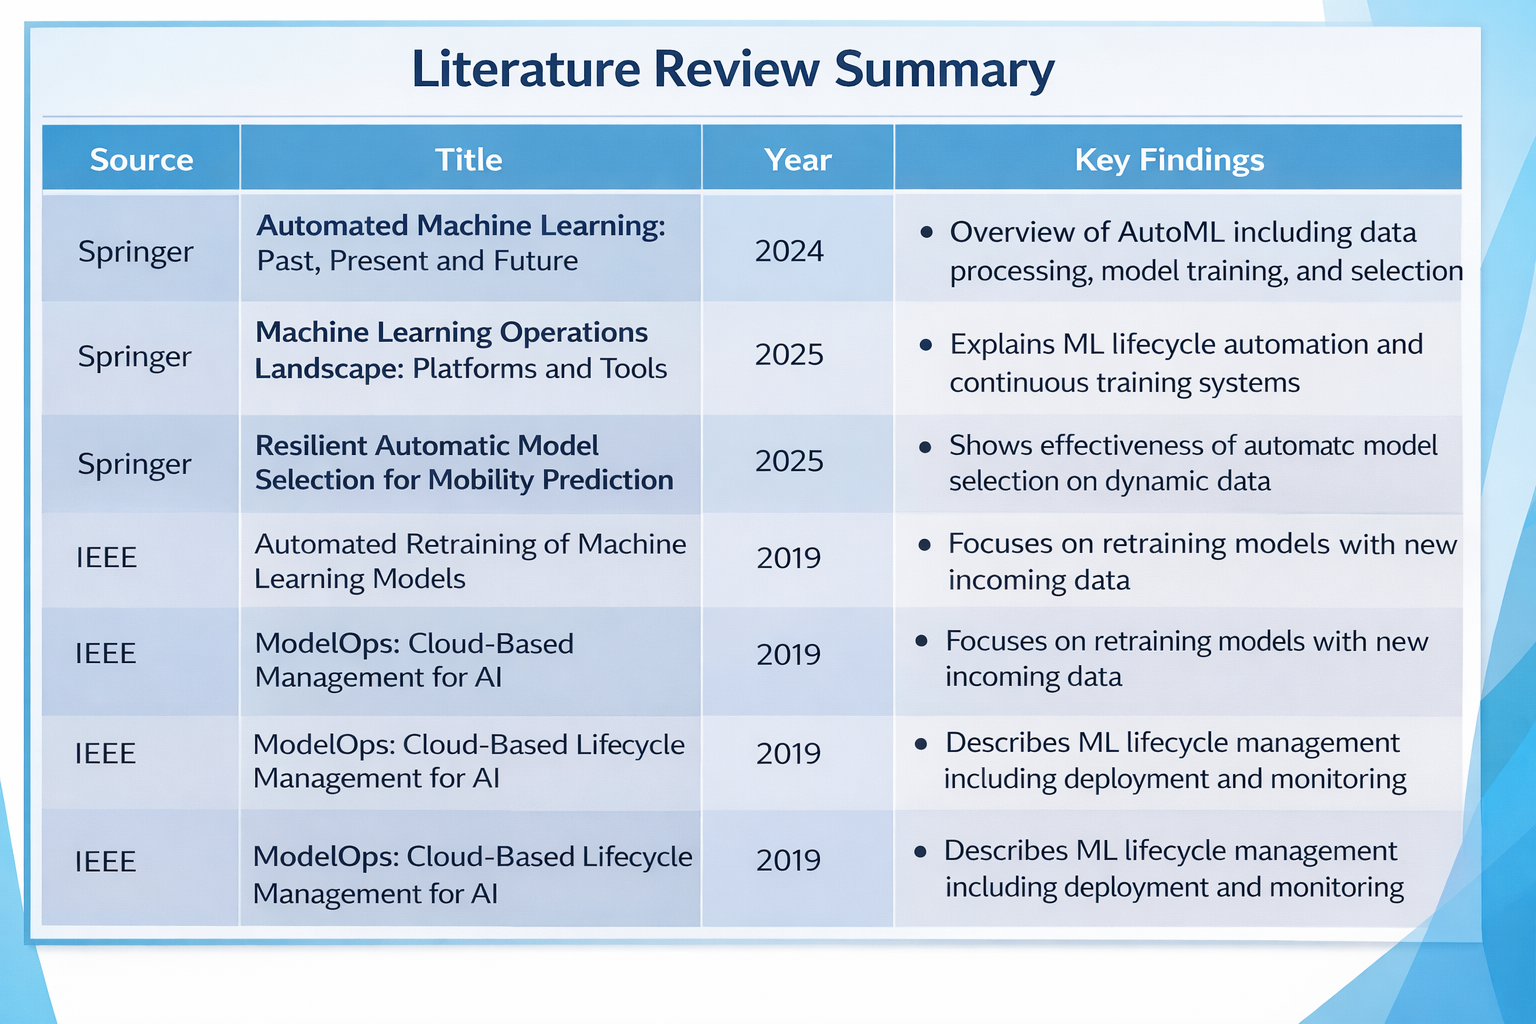
\includegraphics[width=1\textwidth]{images/1.png}}
    \caption{Comparative Analysis of Literature Review}
    \label{fig:img5}
\end{figure}


\chapter{Project Design}
\vspace{-1cm}
\par This section describes how Project Design serves as the foundational blueprint for developing a software solution. It outlines the overall structure, essential features, and technical specifications, guiding the entire development process. The Features and Functionality part details the specific capabilities and user-facing components of the project, explaining what the system will do and how users will interact with it. This comprehensive breakdown of core modules ensures the final product is a centralized and efficient platform that aligns with the project’s goals and user needs. 

\section{Features and Functionality}
\begin{itemize}
\item \textbf{Automatic Data Analysis \& Preprocessing:}

The platform automatically analyzes the structure of uploaded datasets and performs necessary preprocessing steps to prepare the data for training. This includes handling missing values, formatting features, and ensuring the dataset is clean and suitable for machine learning workflows. By automating this process, it reduces manual effort and allows users to focus more on model building rather than data preparation.\\

\item \textbf{Multi-Model Training:}

The system supports training multiple machine learning models simultaneously based on the given dataset. This enables users to explore different algorithms without manually configuring each one, ensuring a comprehensive approach to model development and improving the chances of achieving optimal performance.\\

\item \textbf{Best Model Selection:}

After training multiple models, the platform automatically evaluates their performance and selects the most accurate one. This eliminates the need for manual comparison and ensures that the best-performing model is chosen for further use.\\

\item \textbf{Model Export (.pkl):}

Once the best model is selected, the system generates a reusable \texttt{.pkl} file. This file can be easily integrated into applications or deployed in real-world systems, making the transition from development to production seamless.\\

\item \textbf{Prediction Interface:}

The platform provides a simple and user-friendly interface where users can input data and receive predictions from the trained model. This makes machine learning accessible even to users with minimal technical expertise.\\

\item \textbf{Dataset Upload \& Processing:}

Users can upload their datasets directly to the platform, where the system processes and prepares the data for model training. This feature ensures a smooth and efficient workflow from data ingestion to model development.\\

\item \textbf{Automatic Model Training:}

Based on the type and structure of the dataset, the platform automatically initiates training using suitable machine learning models. This reduces the need for manual configuration and speeds up the development process.\\

\item \textbf{Model Evaluation \& Selection:}

The system evaluates all trained models using relevant performance metrics and compares their results. It then selects the best-performing model, ensuring accuracy and reliability in predictions.\\

\item \textbf{Model Deployment (.pkl):}

The selected model is converted into a deployable \texttt{.pkl} file, allowing users to integrate it into real-world applications, APIs, or systems with ease.\\

\item \textbf{Prediction System:}

The platform enables users to input new data and obtain predictions through an intuitive interface. This feature ensures that the trained model can be effectively used for practical decision-making and real-time applications.\\


\end{itemize}

\vspace{10 cm} 

\section{System Architecture}
\begin{figure}[H]
    \centering
    % Image ko -90 degree rotate kiya gaya hai
    % NOTE: width aur height ki values ko aapas mein badal diya gaya hai
    \fbox{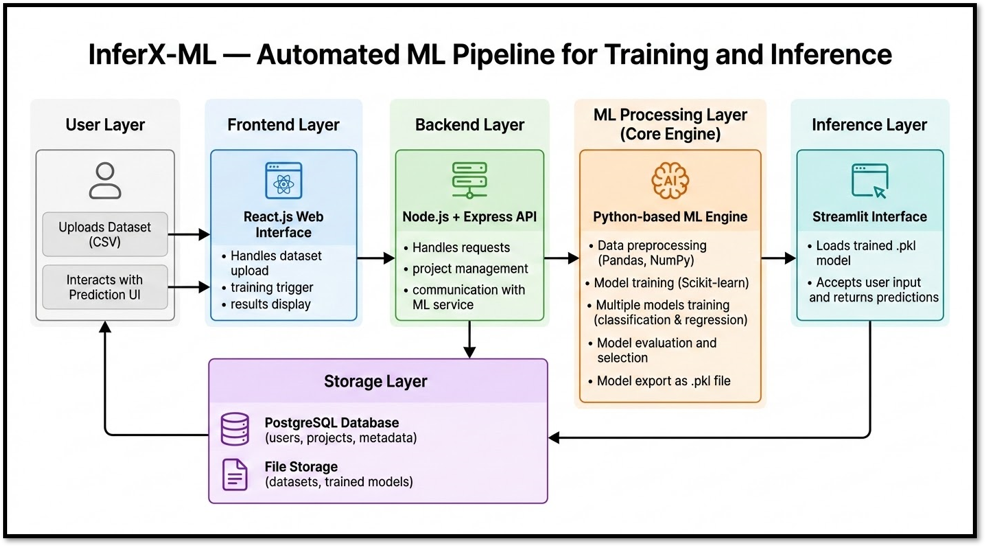
\includegraphics[width=16cm, height=10cm]{images/Designer.png}}
    \caption{System Architecture of InferX-ML}
    \label{fig:image1}
    \vspace{0.2cm}
    \parbox{\textwidth}{\small The diagram illustrates the architecture of InferX-ML, an automated machine learning pipeline that streamlines training and inference. It shows the flow from user interaction through frontend and backend layers to a Python-based ML engine, which handles data preprocessing, model training, and selection. The system stores data and models efficiently and provides predictions through an inference layer using a simple user interface.}
\end{figure}

\vspace{10 cm}

\section{DFD (Data Flow Diagrams)}
\begin{figure}[H]
    \centering
    \fbox{\includegraphics[width=17cm, height=3.5cm]{images/dfd-0.png}}
    \caption{Data flow Diagram of InferX-ML (Level 0)}
    \label{fig:image2}
 \vspace{0.2cm} % Adds a small space after the caption
    \parbox{\textwidth}{\small This Data Flow Diagram (DFD) at Level 0 represents the overall system context for the InferX-ML platform, where the User interacts with the central system to upload data, train models, and generate predictions, while the platform processes requests through its backend, ML engine, and storage, and integrates with external AI services like the Gemini API to deliver insights.}
\end{figure}

\begin{figure}[H]
    \centering
    \fbox{\includegraphics[width=17cm, height=7cm]{images/dfd-2.png}}
    \caption{Data flow Diagram of InferX-ML  (Level 1)}
    \label{fig:image2}
\vspace{0.2cm} % Adds a small space after the caption
    \parbox{\textwidth}{\small This Data Flow Diagram (DFD) at Level 1 represents the detailed workflow of the InferX-ML platform, where the User interacts with modules like authentication, dataset management, training orchestration, and the ML engine to build and deploy models, while data and models are stored in PostgreSQL and MinIO, and the AI Insight Layer integrates with the Gemini API to generate explainable, human-readable insights.}
\end{figure}

\begin{figure}[H]
    \centering
    \fbox{\includegraphics[width=17cm, height=5.5cm]{images/dfd-1.png}}
    \caption{Data flow Diagram of InferX-ML (Level 2)}
    \label{fig:image2}
\vspace{0.2cm} % Adds a small space after the caption
    \parbox{\textwidth}{\small This Data Flow Diagram (DFD) at Level 2 represents the modular architecture of the InferX-ML platform, where the User interacts with distinct microservices such as Auth, Dataset Management, Training, ML Engine, and Prediction services, each connected to dedicated storage systems (PostgreSQL and MinIO), while the AI Insight Layer integrates with the Gemini API to generate intelligent insights.
}
\end{figure}

\section{Use Case Diagram}
\begin{figure}[H]
    \centering
    \fbox{\includegraphics[width=15cm, height=20cm]{images/new.png}}
    \caption{Use Case Diagram of InferX-ML}
    \label{fig:img5}
\vspace{0.2cm} % Adds a small space after the caption
    \parbox{\textwidth}{\small A use-case diagram of an AI Model Training Platform showing subsystems like authentication, dataset management, training, model management, and prediction.
It illustrates how a user interacts with these components and integrates external AI services (Gemini API) for analysis and insights.}
\end{figure}


\chapter{Technical Specification}
\vspace{-1cm}

The technical architecture and technology stack used in the development, deployment, and maintenance of InferX-ML are described herein. The platform follows a modern microservices-based architecture integrating a React-based frontend, a Flask-powered backend, and a modular machine learning engine. PostgreSQL is leveraged for relational data storage and MinIO for scalable object storage. The entire system is containerized using Docker and orchestrated via Docker Compose, ensuring reproducibility and ease of deployment.


\section{Front-End (Client-Side)}

\begin{description}
\item[React JS :] Used to build an interactive interfaces.
\item[Vite :] Provides fast development server, hot module replacement, and optimized builds.
\item[Tailwind CSS :] Used for responsive UI design and styling.
\item[React Router :] Enables seamless navigation across different pages.
\item[Zustand :] Manages global state such as authentication and sessions.
\item[Axios :] Used for REST API communication with the backend.
\item[Streamlit :] Provides ML-specific interfaces.
\end{description}


\section{Back-End (Server-Side)}

\begin{description}
\item[Python :] Core programming language for backend and ML engine.
\item[Flask :] REST API framework for managing datasets, training workflows, and predictions.
\item[SQLAlchemy :] ORM for database interaction and schema management.
\item[Celery :] Handles asynchronous model training tasks.
\item[Redis :] Message broker for task queues and caching.
\item[PostgreSQL :] Stores user data, experiments, and model metadata.
\item[MinIO :] Object storage for datasets, models, and artifacts.
\end{description}


\section{Machine Learning Engine}

\begin{description}
\item[Pandas \& NumPy :] Used for data preprocessing and operations.
\item[Scikit-learn \& XGBoost :] Provide various algorithms.
\item[TensorFlow / Keras :] Used for deep learning models and image classification.
\item[Prophet \& Statsmodels :] Used for time-series forecasting.
\item[SHAP :] Provides model explainability and feature importance insights.
\item[Joblib / Pickle :] Used for model serialization and deployment.
\end{description}


\section{Development, Operations and Deployment}

\begin{description}
\item[Docker :] Containerizes all services for consistent environments.
\item[Docker Compose :] Manages multi-container application deployment.
\item[Nginx :] Acts as a reverse proxy for routing and serving frontend.
\item[Git \& GitHub :] Used for version control and collaboration.
\end{description}


\section{Development Tools}

\begin{description}
\item[Visual Studio Code :] Primary development environment.
\item[npm \& pip :] Manage frontend and backend dependencies.
\item[Postman :] Used for API testing and debugging.
\item[pytest :] Used for testing backend and ML pipelines.
\end{description}
\chapter{Project Implementation}

\vspace{-1cm}

Building a functional machine learning platform requires translating architectural blueprints and design specifications into production-quality code through systematic coding, integration, and rigorous testing. The following screenshots present key portions of the InferX-ML interface, along with explanations of their purpose and role in the overall system.

\section{Code Snippets}
\begin{figure}[H]
    \centering
    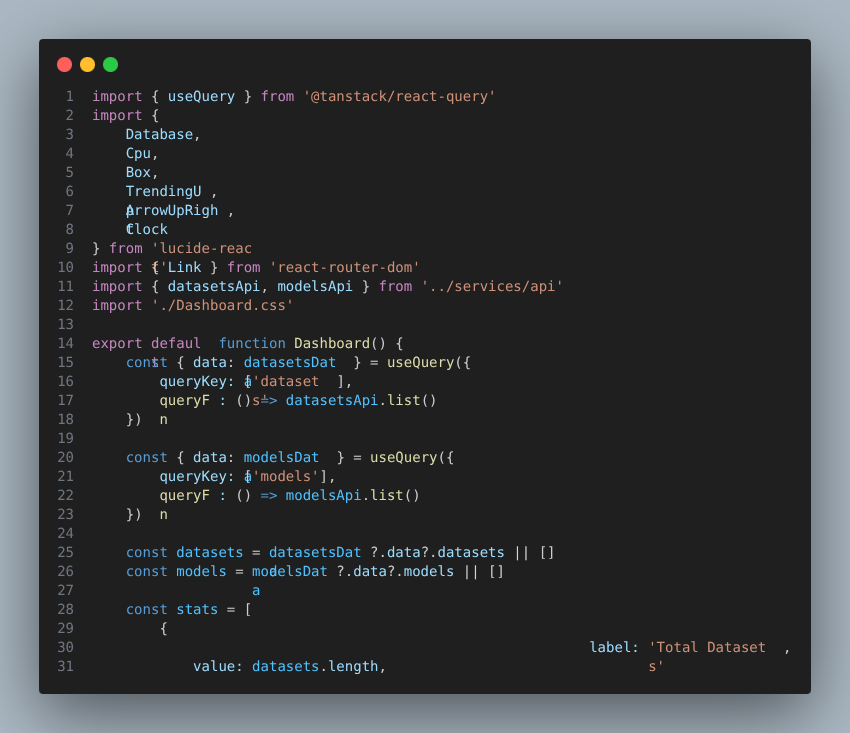
\includegraphics[width=0.8\textwidth]{images/4.1.png}
    \caption{Home Page}
    \label{fig:fig1}
    \vspace{0.2cm}
    \parbox{\textwidth}{\small Displays an overview of the platform with summary statistics (total datasets, trained models, training jobs, predictions), quick action shortcuts, and a list of recently trained models.}
\end{figure}

\begin{figure}[H]
    \centering
    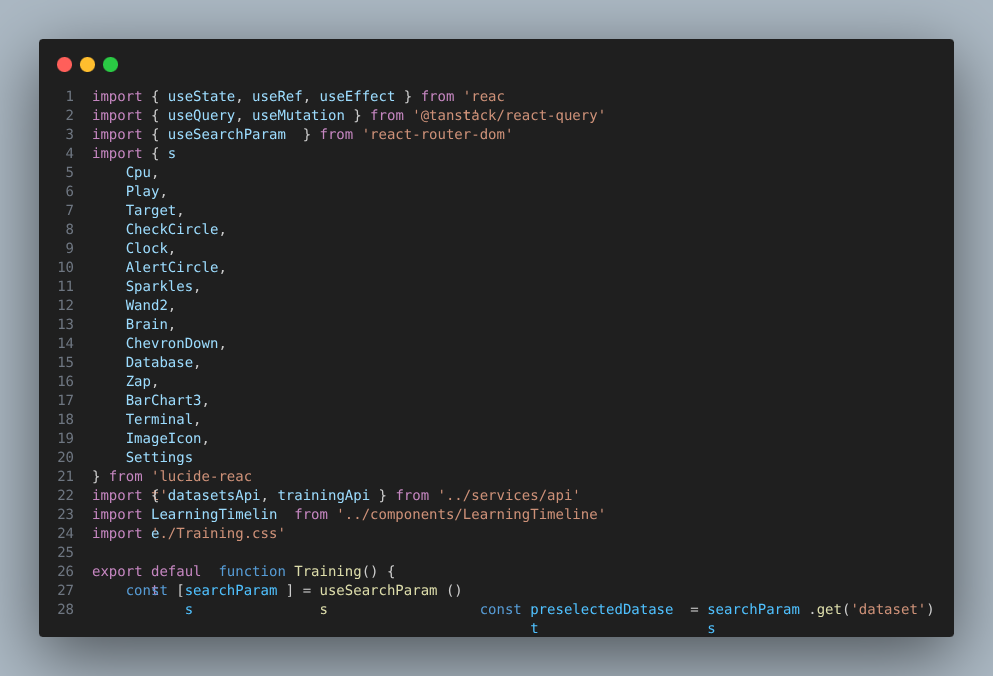
\includegraphics[width=0.8\textwidth]{images/3.1.png}
    \caption{Training Page}
    \label{fig:fig2}
    \vspace{0.2cm}
    \parbox{\textwidth}{\small Allows users to configure and launch AutoML training jobs by selecting a dataset, optionally using AI-powered goal analysis to suggest a target column, setting advanced hyperparameters, and monitoring real-time training logs and pipeline progress.}
\end{figure}

\begin{figure}[H]
    \centering
    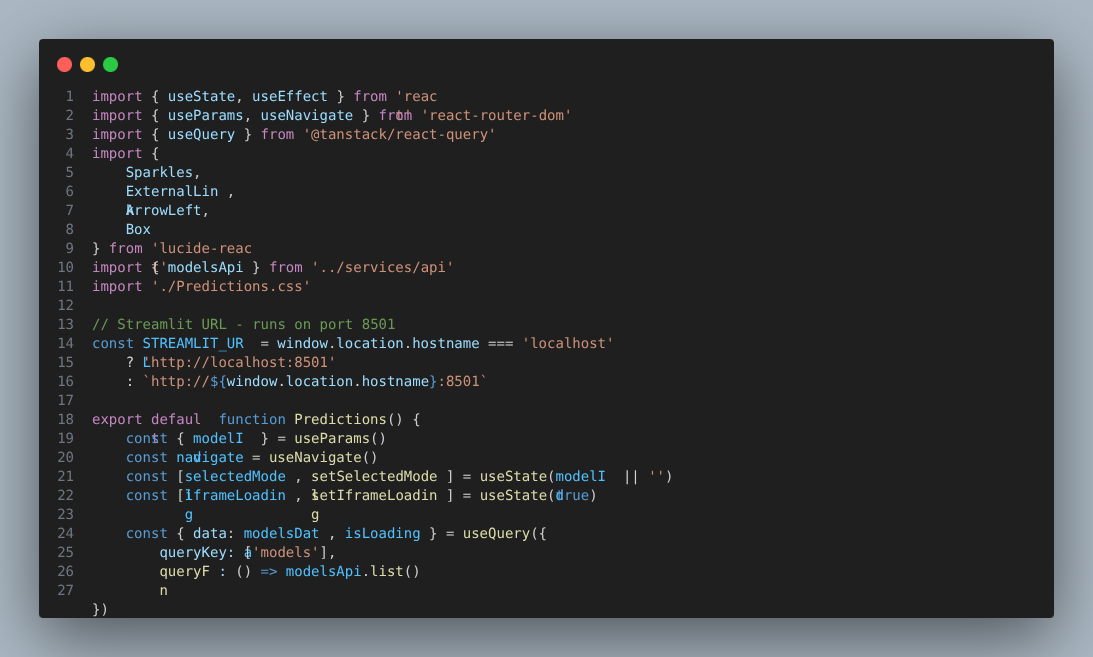
\includegraphics[width=0.8\textwidth]{images/5.png}
    \caption{Prediction Page}
    \label{fig:fig3}
    \vspace{0.2cm}
    \parbox{\textwidth}{\small Lets users select a trained model and make predictions through an embedded Streamlit interface loaded in an iframe, with options to open it in a new tab.}
\end{figure}

% ===================== REPLACED SECTION =====================

\newpage
\section{Cost Estimation using COCOMO Model}

\noindent\textbf{Project Type}
\begin{itemize}
    \item Organic Mode
\end{itemize}

\vspace{0.3cm}
\noindent\textbf{Assumptions}
\begin{itemize}
    \item Size = 10 KLOC
\end{itemize}

\vspace{0.3cm}
\noindent\textbf{Effort Estimation}

The effort is calculated using the basic COCOMO formula:
\[
E = 2.4 \times (KLOC)^{1.05}
\]

\[
E = 2.4 \times (10)^{1.05} \approx 27 \text{ Person-Months}
\]

\vspace{0.3cm}
\noindent\textbf{Development Time}

The development time is calculated as:
\[
D = 2.5 \times (E)^{0.38}
\]

\[
D = 2.5 \times (27)^{0.38} \approx 8 \text{ Months}
\]

\vspace{0.3cm}
\noindent\textbf{Cost Estimation}

\begin{itemize}
    \item Cost per person per month = Rs. 15,000
    \item Total Cost = $27 \times 15,000 = \text{Rs. } 4,05,000 \approx 4$ Lakhs
\end{itemize}

\vspace{0.3cm}
\noindent\textbf{Conclusion}

\begin{itemize}
    \item Effort: $\sim 27$ Person-Months
    \item Time: $\sim 8$ Months
    \item Team Size: 3--4 Members
\end{itemize}

% ===================== END =====================
\chapter{Project Scheduling}

\vspace{-1cm}

The visual timeline below illustrates the strategic execution and delivery phases of the InferX-ML platform. Orchestrated over a multi-month development cycle, the schedule emphasizes a modular approach to building, integrating, and validating the automated machine learning engine and its corresponding user interface.

\begin{figure}[H]
    \centering
    \fbox{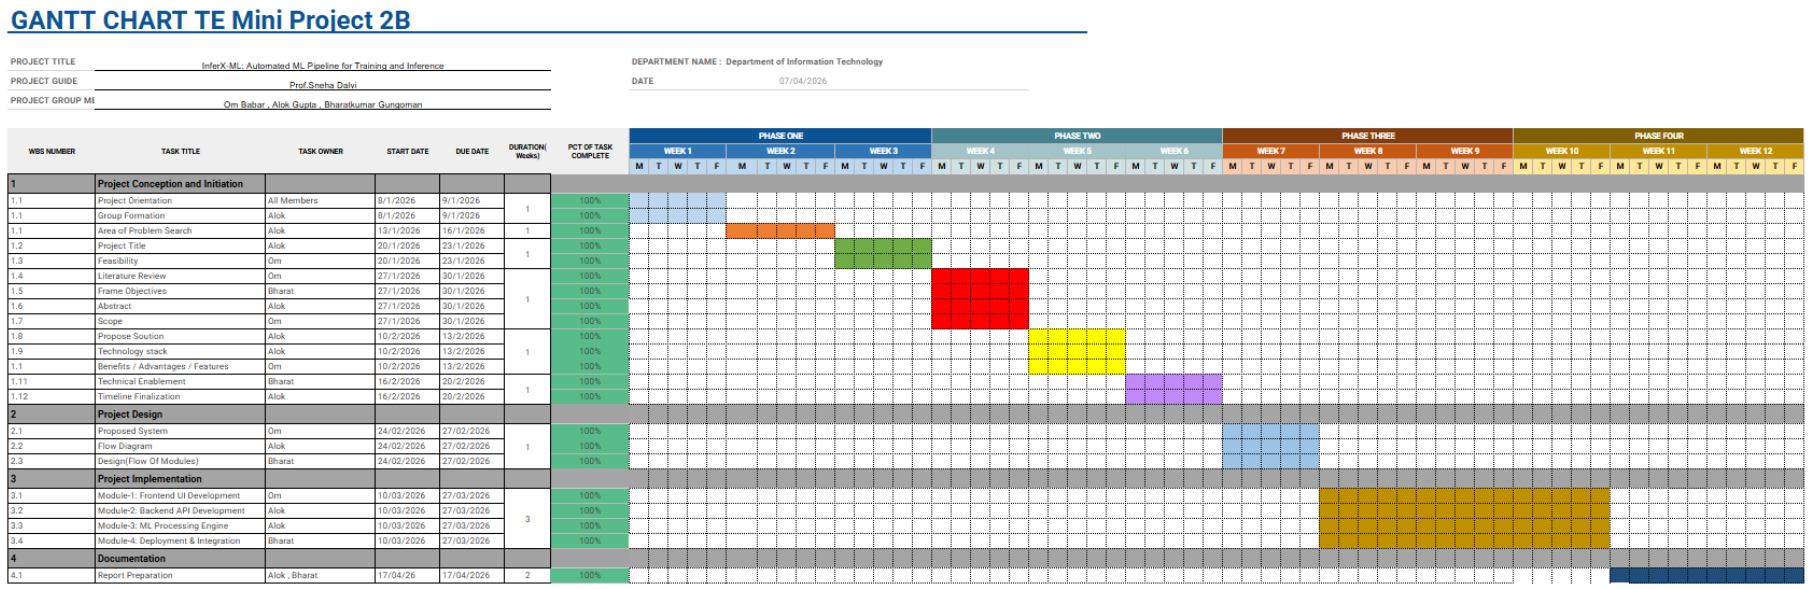
\includegraphics[width=1.0\textwidth]{images/Gantt-Chat.png}}
    \caption{Project Scheduling - Gantt Chart}
    \label{fig:gantt_chart}
\end{figure}

\vspace{0.2cm}
The scheduling highlights the logical progression from initial conceptualization and architectural design to the parallel development of core ML modules and backend Flask services. The final phases focus on seamless platform integration, rigorous automated pipeline testing, and the deployment of the responsive interface, ensuring a high-performance and reliable end-to-end user experience.

\chapter{Results }\vspace{-1cm}

This chapter showcases the final outcome of the development process. The results are presented as a series of screenshots that provide a visual tour of the completed web application. These images display the user interface (UI) of various key pages, demonstrating the successful implementation of the project's core functionalities and features as outlined in the design phase.
\setlength{\fboxsep}{0pt} % no space between image and border

\begin{figure}[H]
    \centering
    \fbox{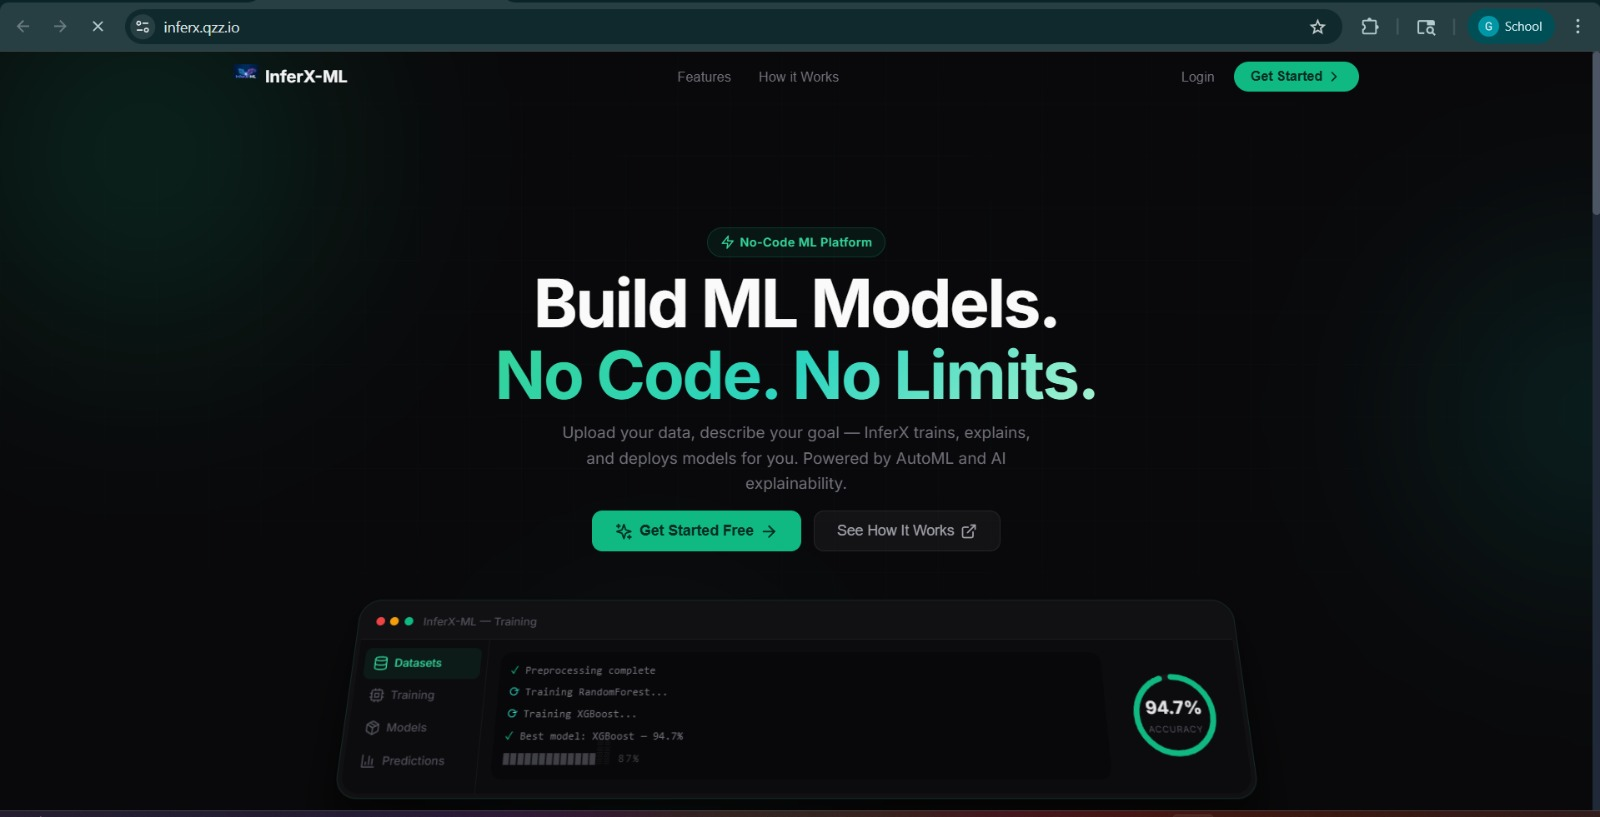
\includegraphics[width=0.8\textwidth]{images/1.jpeg}}
    \caption{Home Page}
    \label{fig:img4}
\end{figure}

\begin{figure}[H]
    \centering
    \fbox{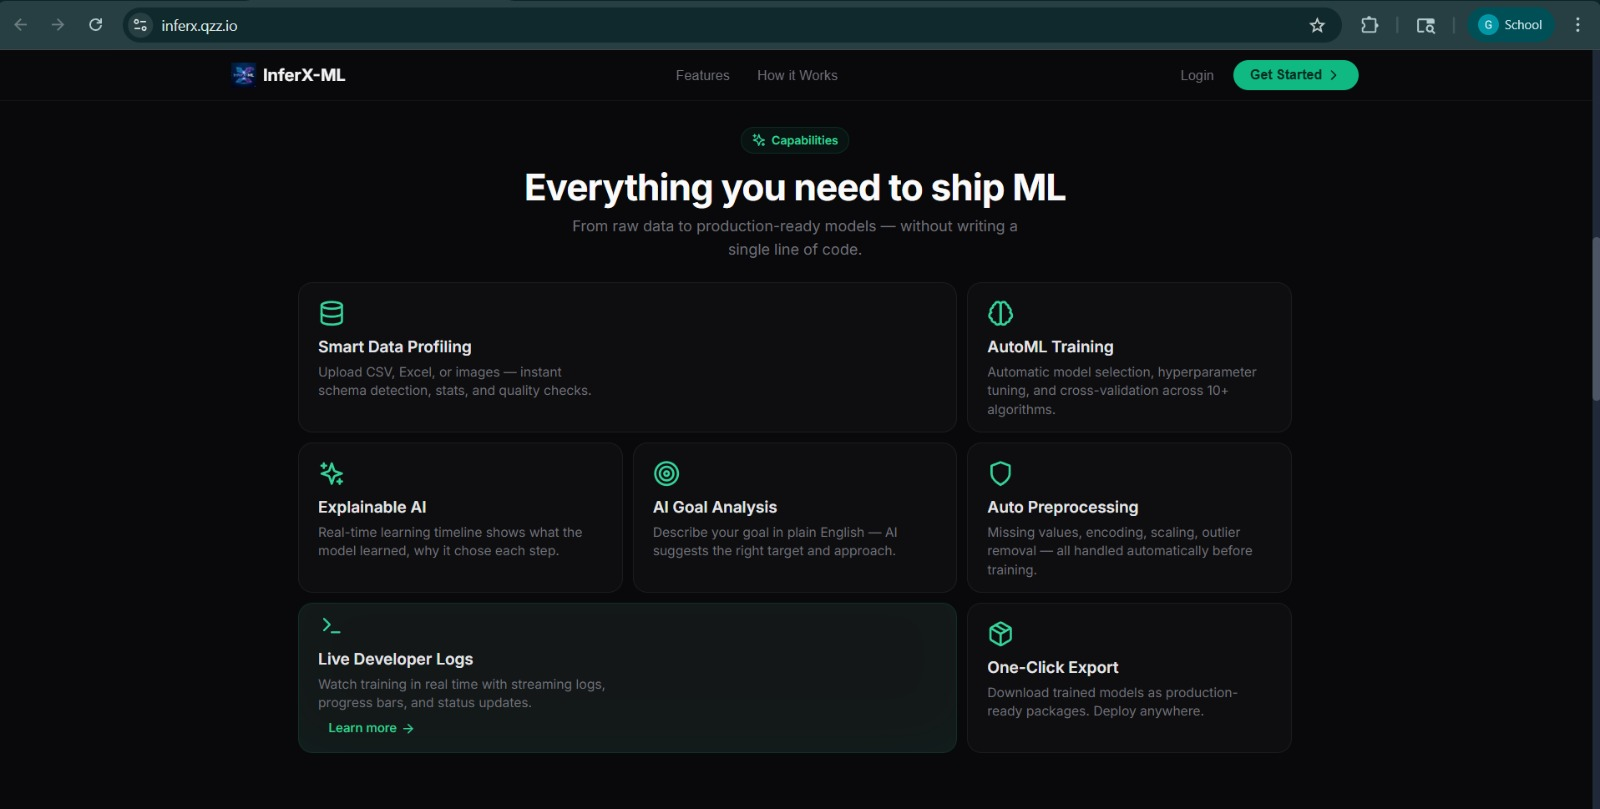
\includegraphics[width=0.8\textwidth]{images/2.jpeg}}
    \caption{AutoML Features}
    \label{fig:img5}
\end{figure}

\begin{figure}[H]
    \centering
    \fbox{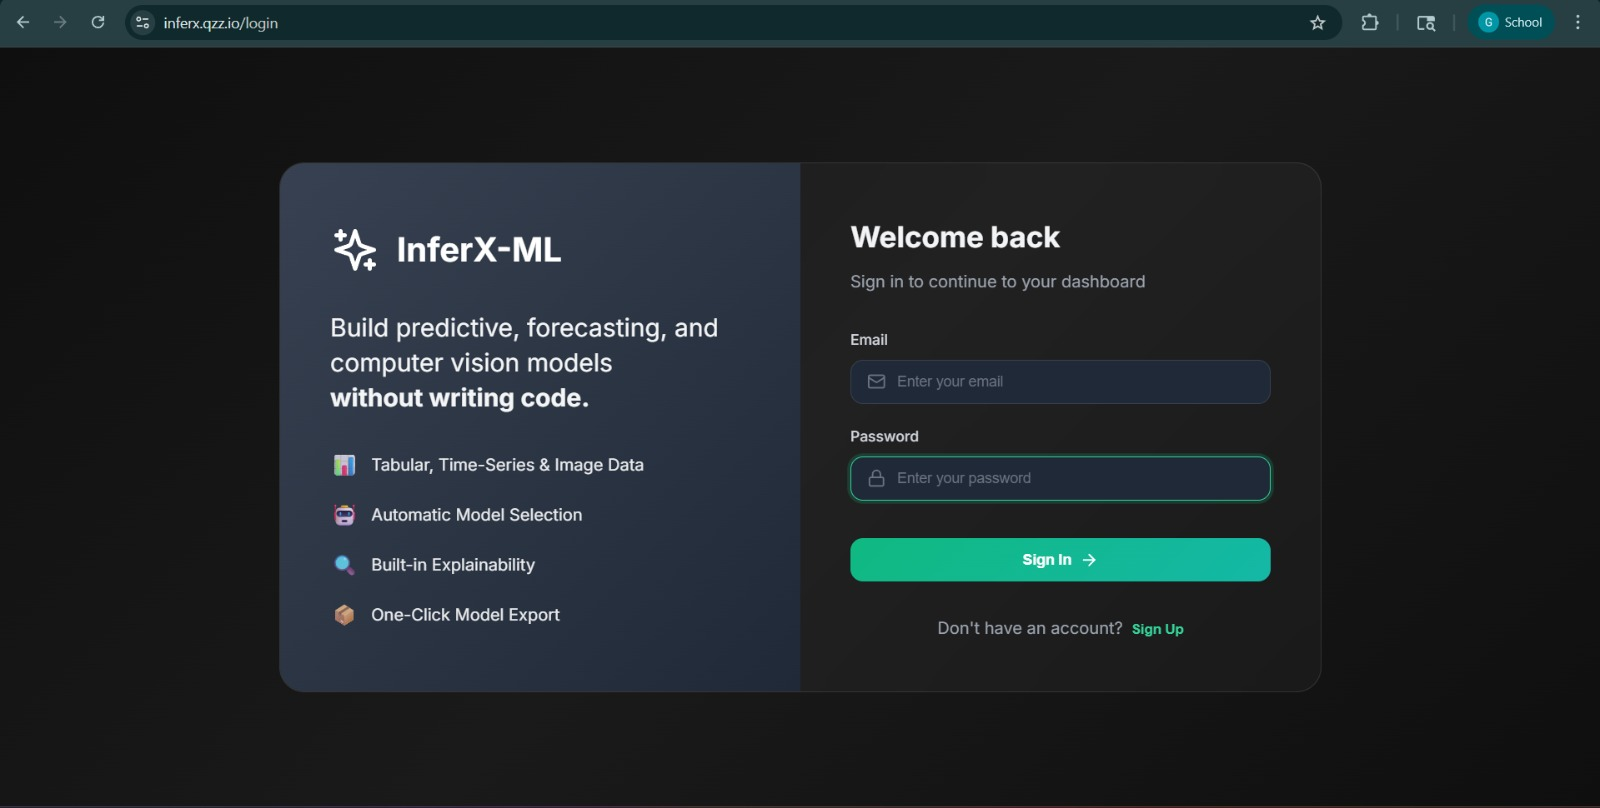
\includegraphics[width=0.8\textwidth]{images/3.jpeg}}
    \caption{Login Page}
    \label{fig:img6}
\end{figure}

\begin{figure}[H]
    \centering
    \fbox{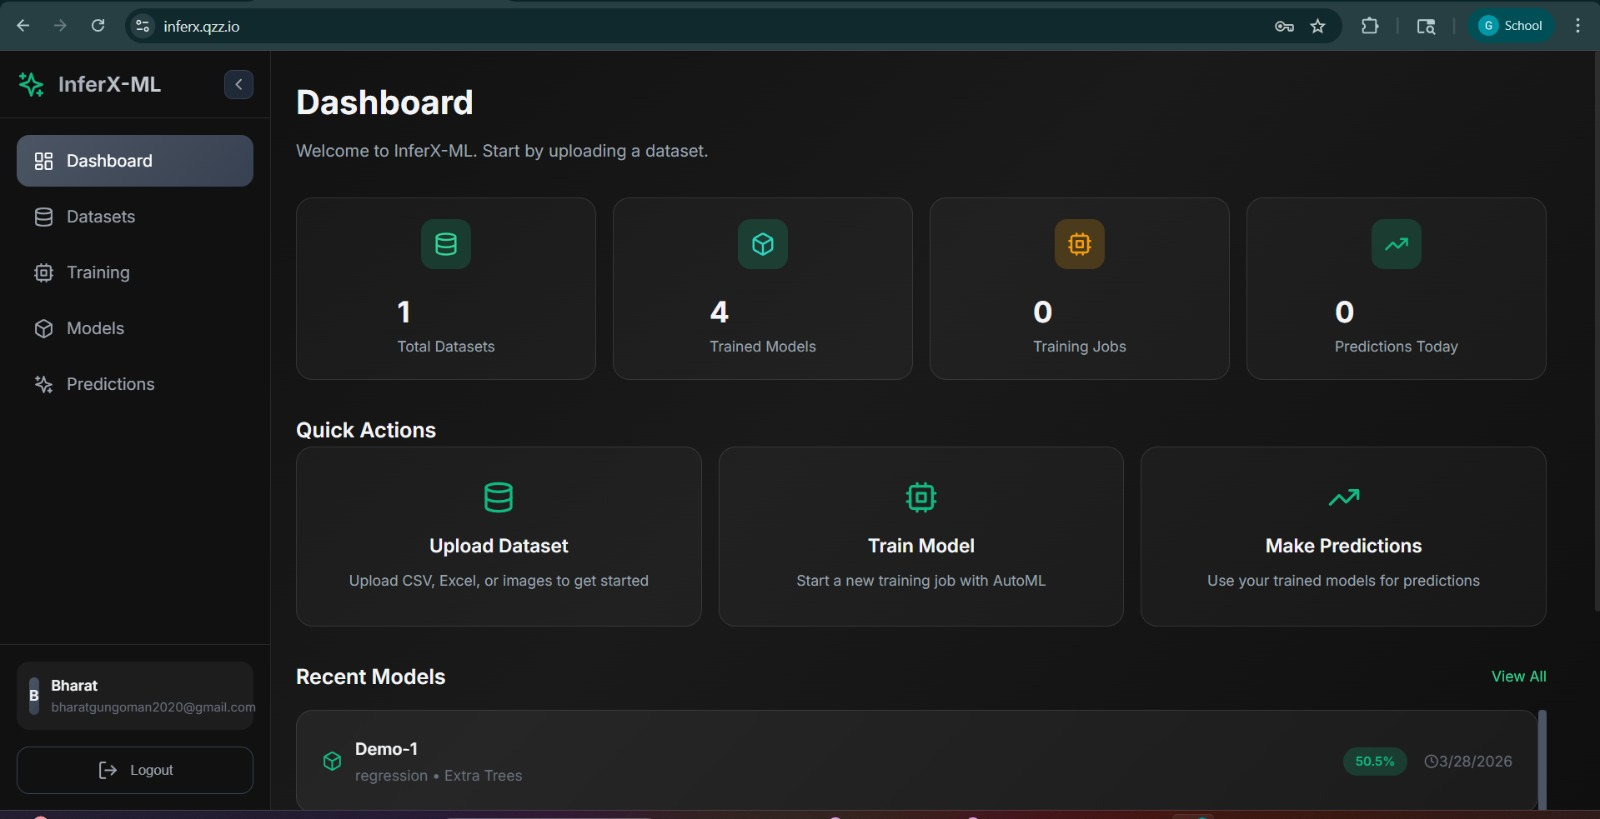
\includegraphics[width=0.8\textwidth]{images/4.jpeg}}
    \caption{Dashboard Page}
    \label{fig:img7}
\end{figure}

\begin{figure}[H]
    \centering
    \fbox{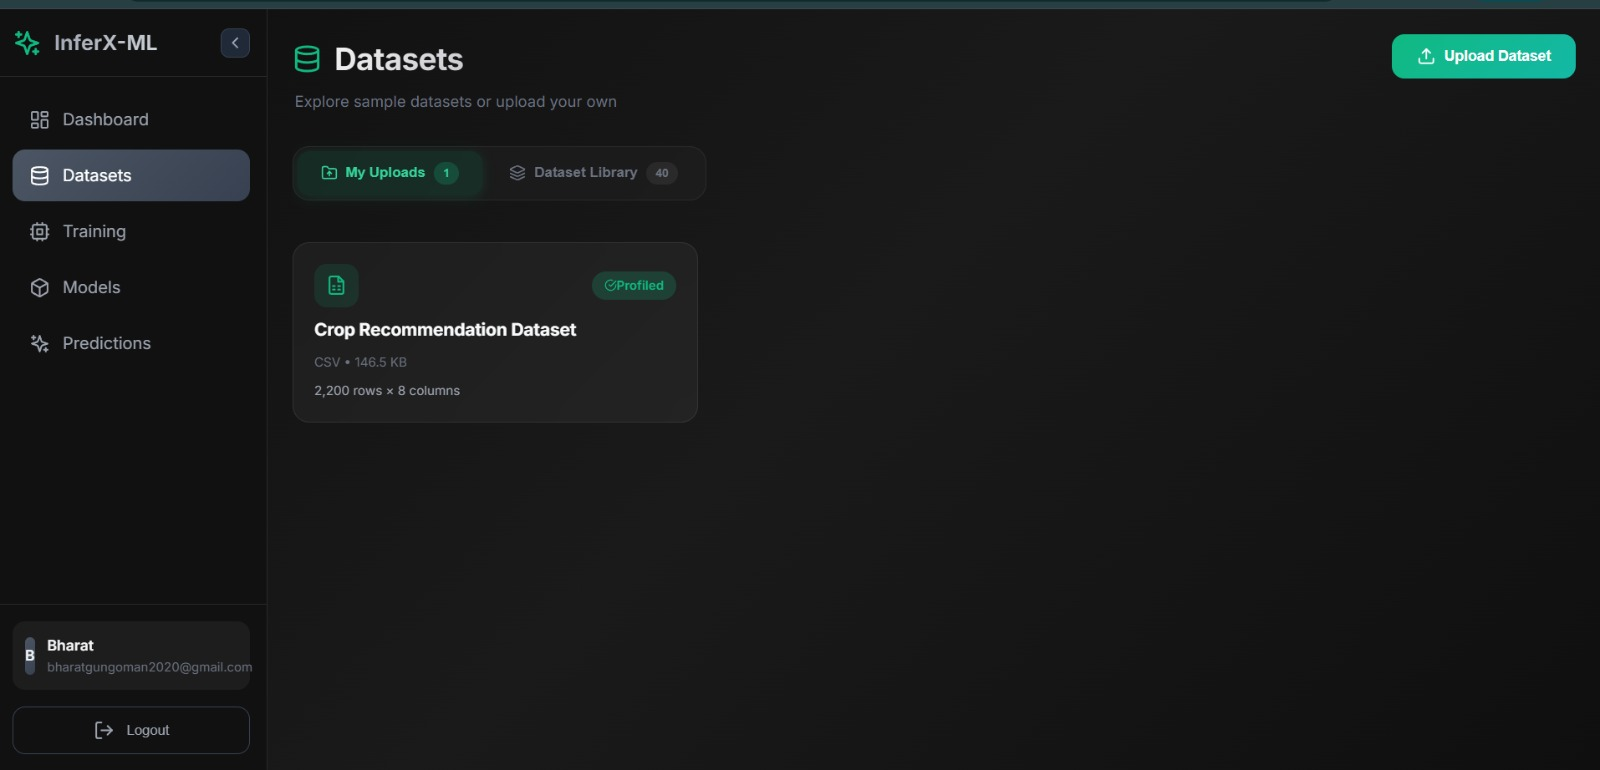
\includegraphics[width=0.8\textwidth]{images/5.jpeg}}
    \caption{Dataset Preview Page}
    \label{fig:img7}
\end{figure}

\begin{figure}[H]
    \centering
    \fbox{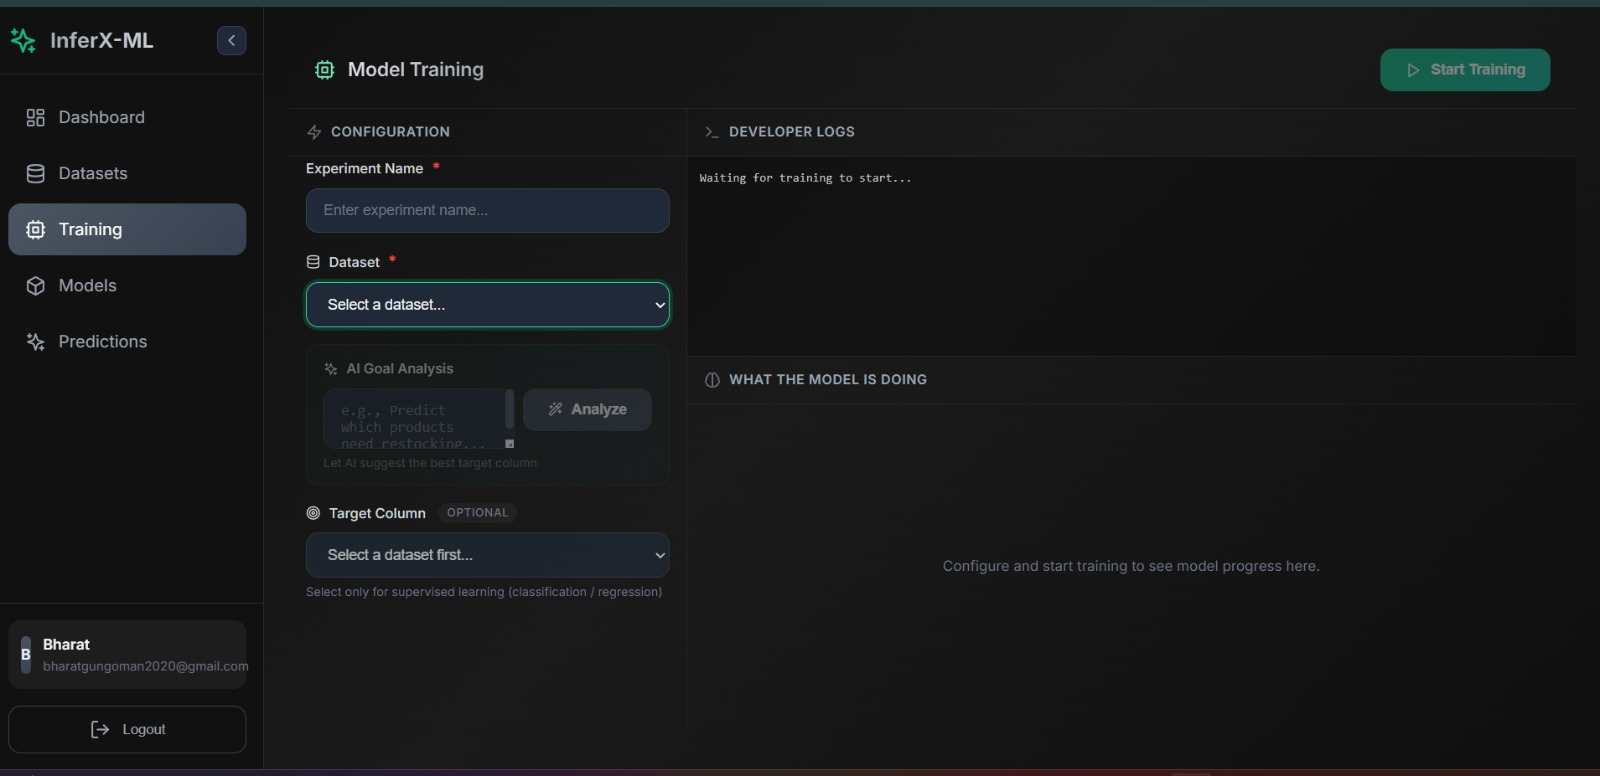
\includegraphics[width=15cm, height=10cm]{images/6.jpeg}}
    \caption{Model Training Page}
    \label{fig:img7}
\end{figure}

\begin{figure}[H]
    \centering
    \fbox{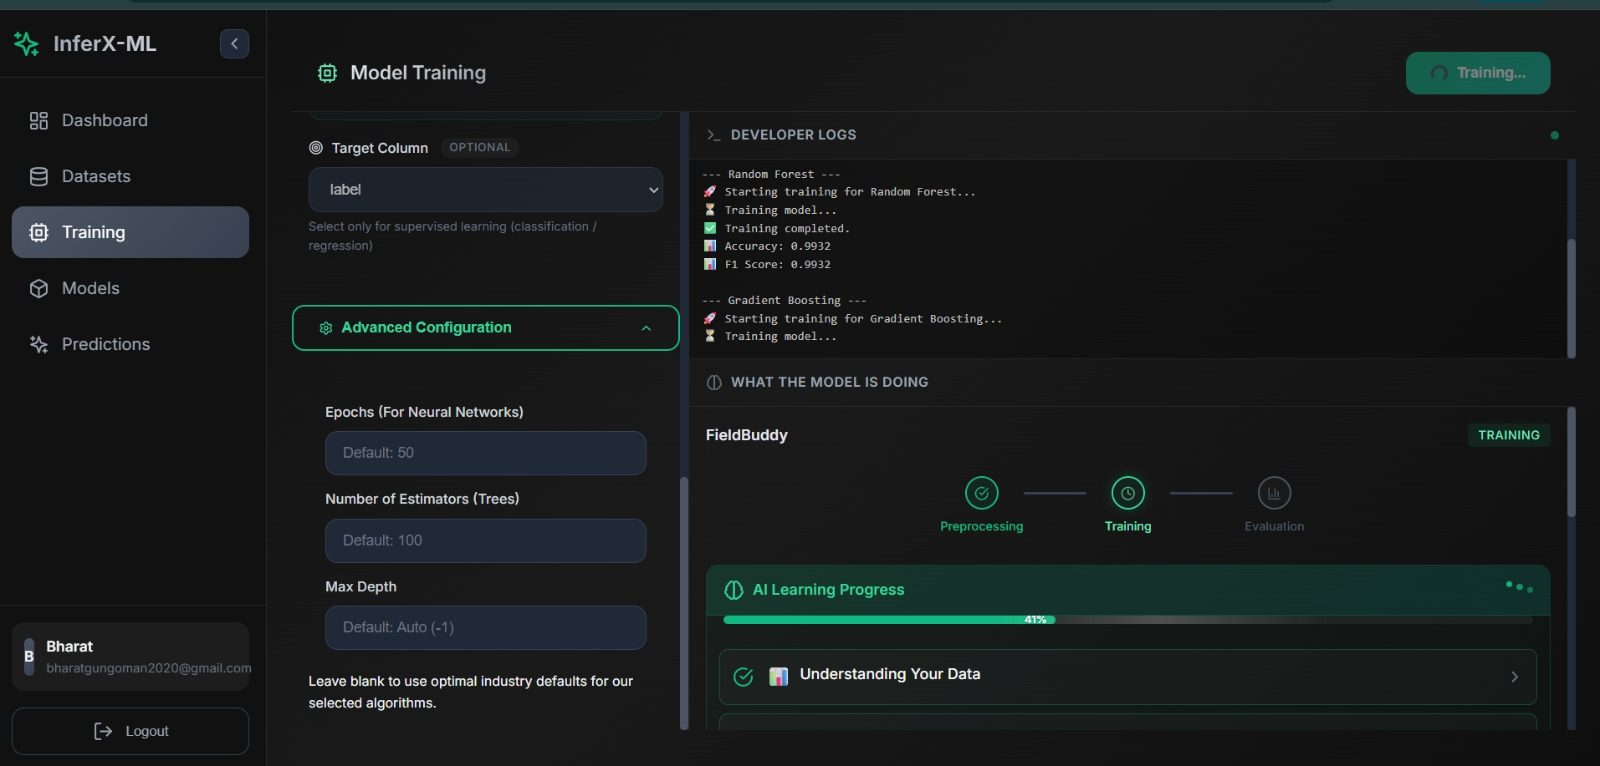
\includegraphics[width=0.8\textwidth]{images/7.jpeg}}
    \caption{AutoML Pipeline Page}
    \label{fig:img7}
\end{figure}

\begin{figure}[H]
    \centering
    \fbox{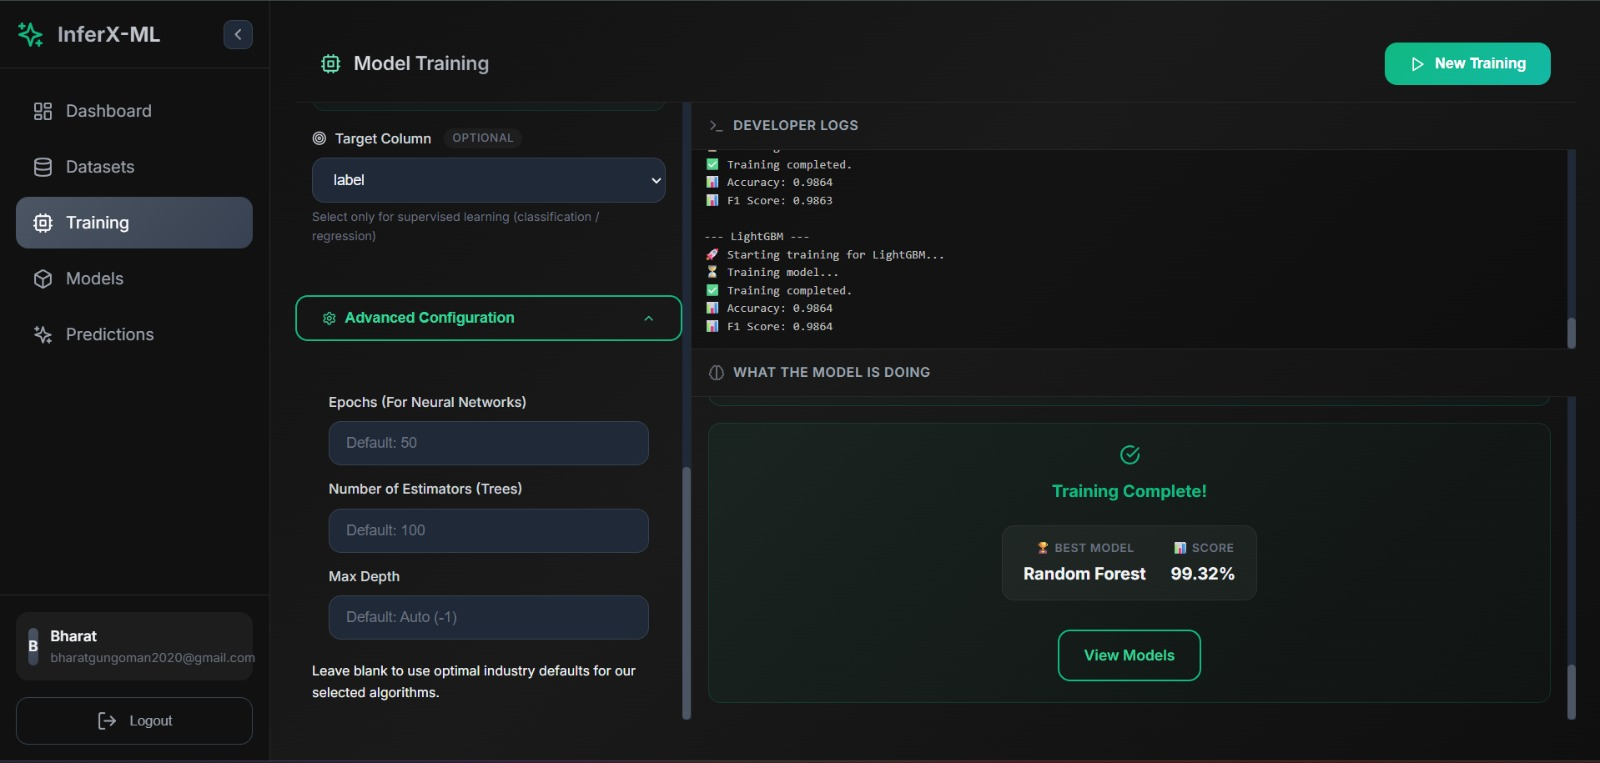
\includegraphics[width=1\textwidth]{images/8.jpeg}}
    \caption{Model Training}
    \label{fig:img7}
\end{figure}

\begin{figure}[H]
    \centering
    \fbox{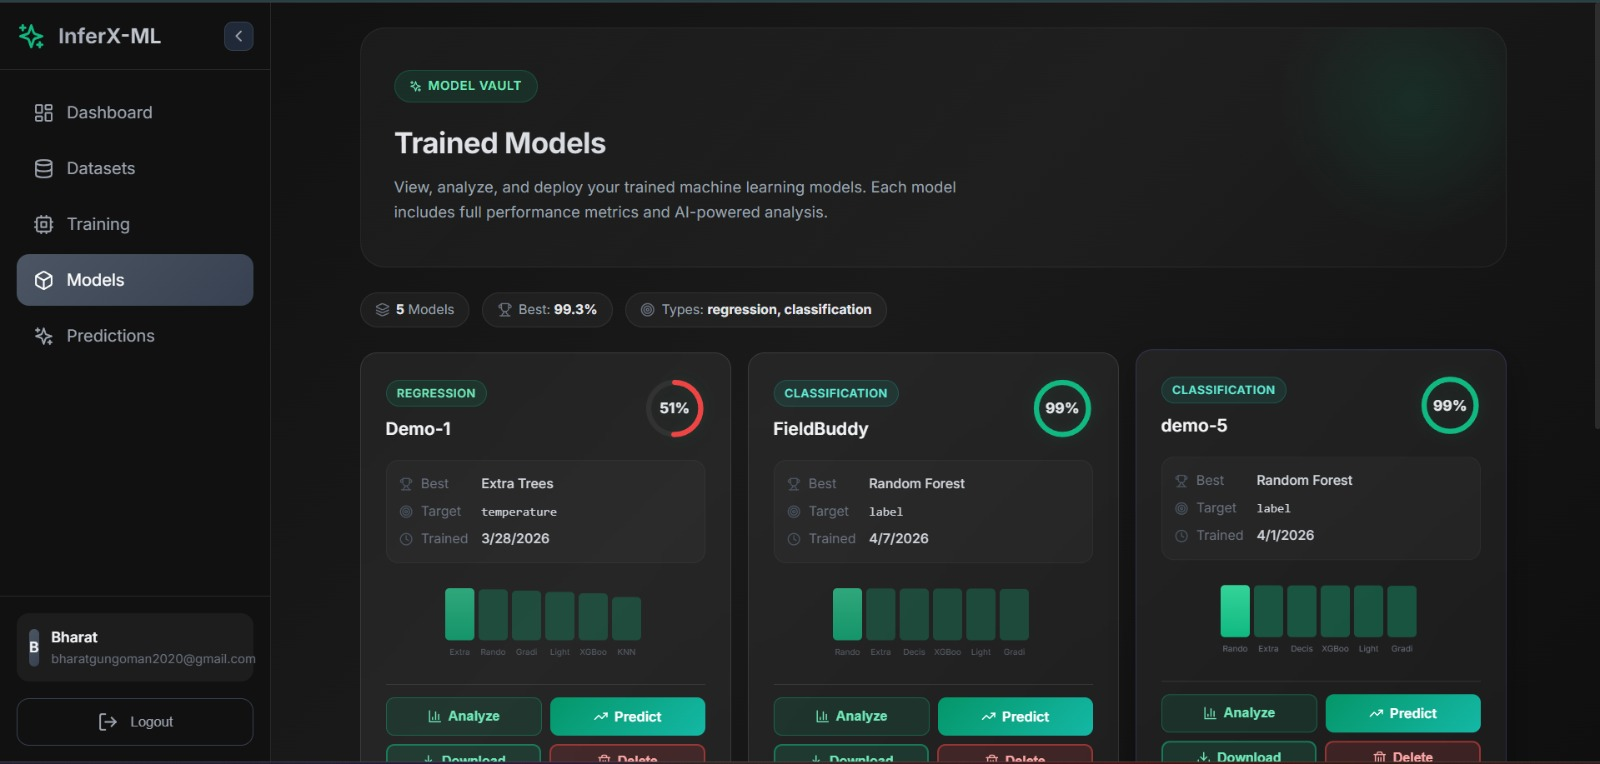
\includegraphics[width=1\textwidth]{images/9.jpeg}}
    \caption{Available Trained Models}
    \label{fig:img7}
\end{figure}

\begin{figure}[H]
    \centering
    \fbox{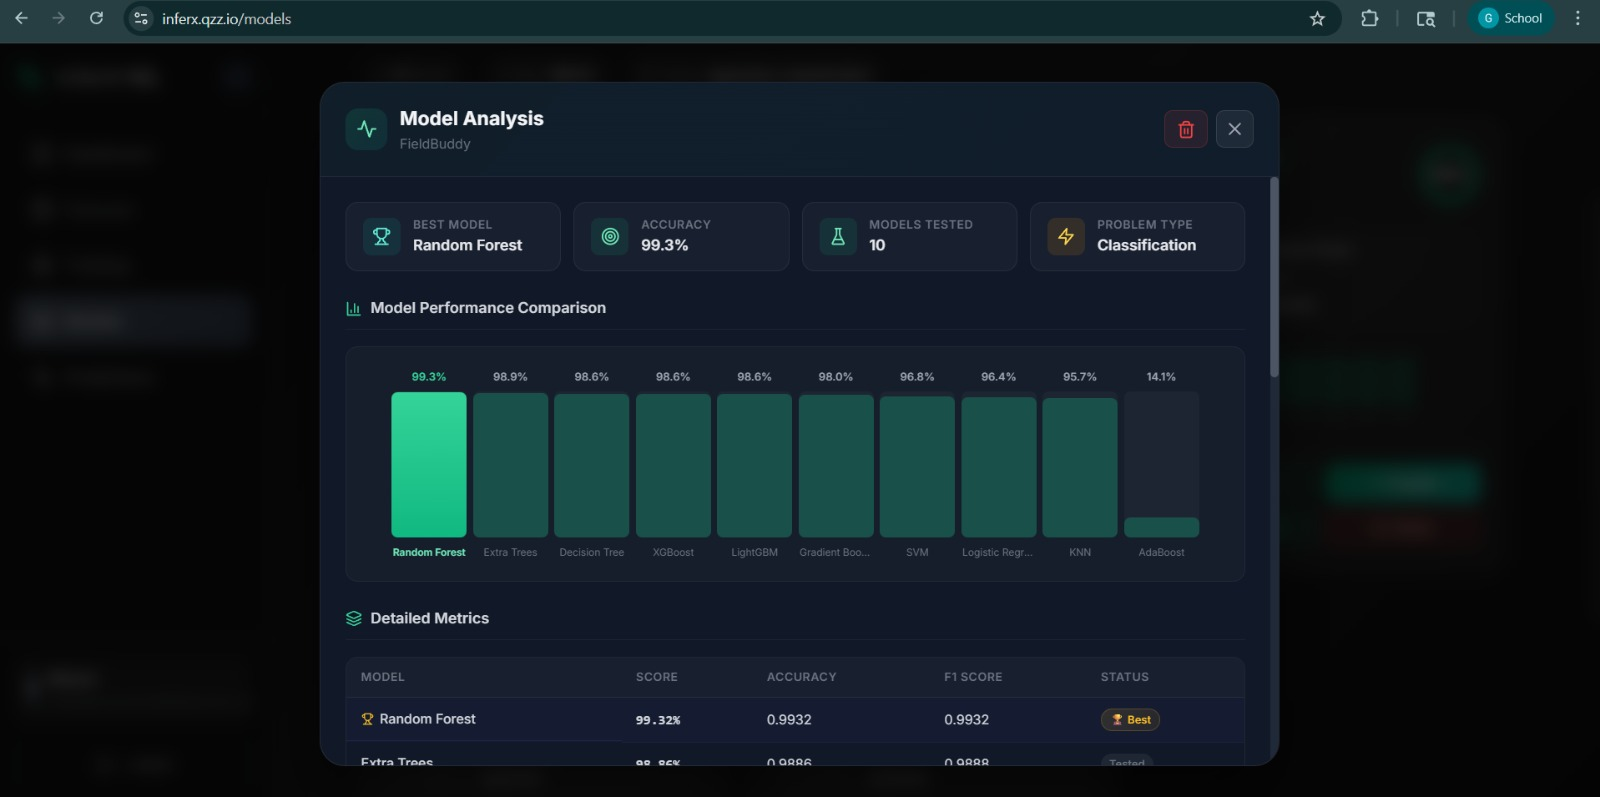
\includegraphics[width=1\textwidth]{images/12.jpeg}}
    \caption{Model Analysis Page}
    \label{fig:img7}
\end{figure}

\begin{figure}[H]
    \centering
    \fbox{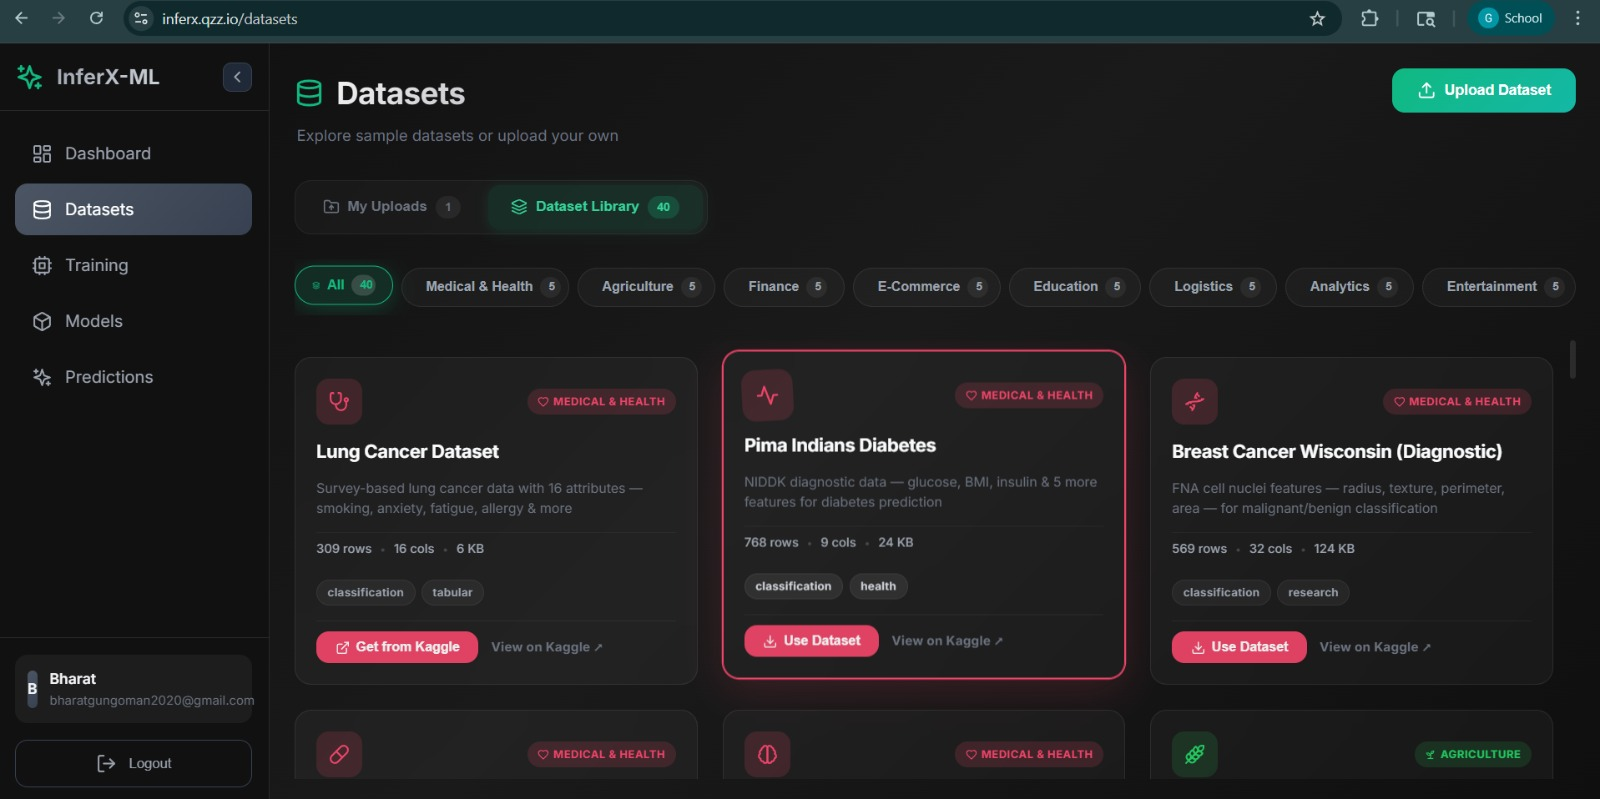
\includegraphics[width=1\textwidth]{images/13.jpeg}}
    \caption{Dataset Preview Page}
    \label{fig:img7}
\end{figure}

\begin{figure}[H]
    \centering
    \fbox{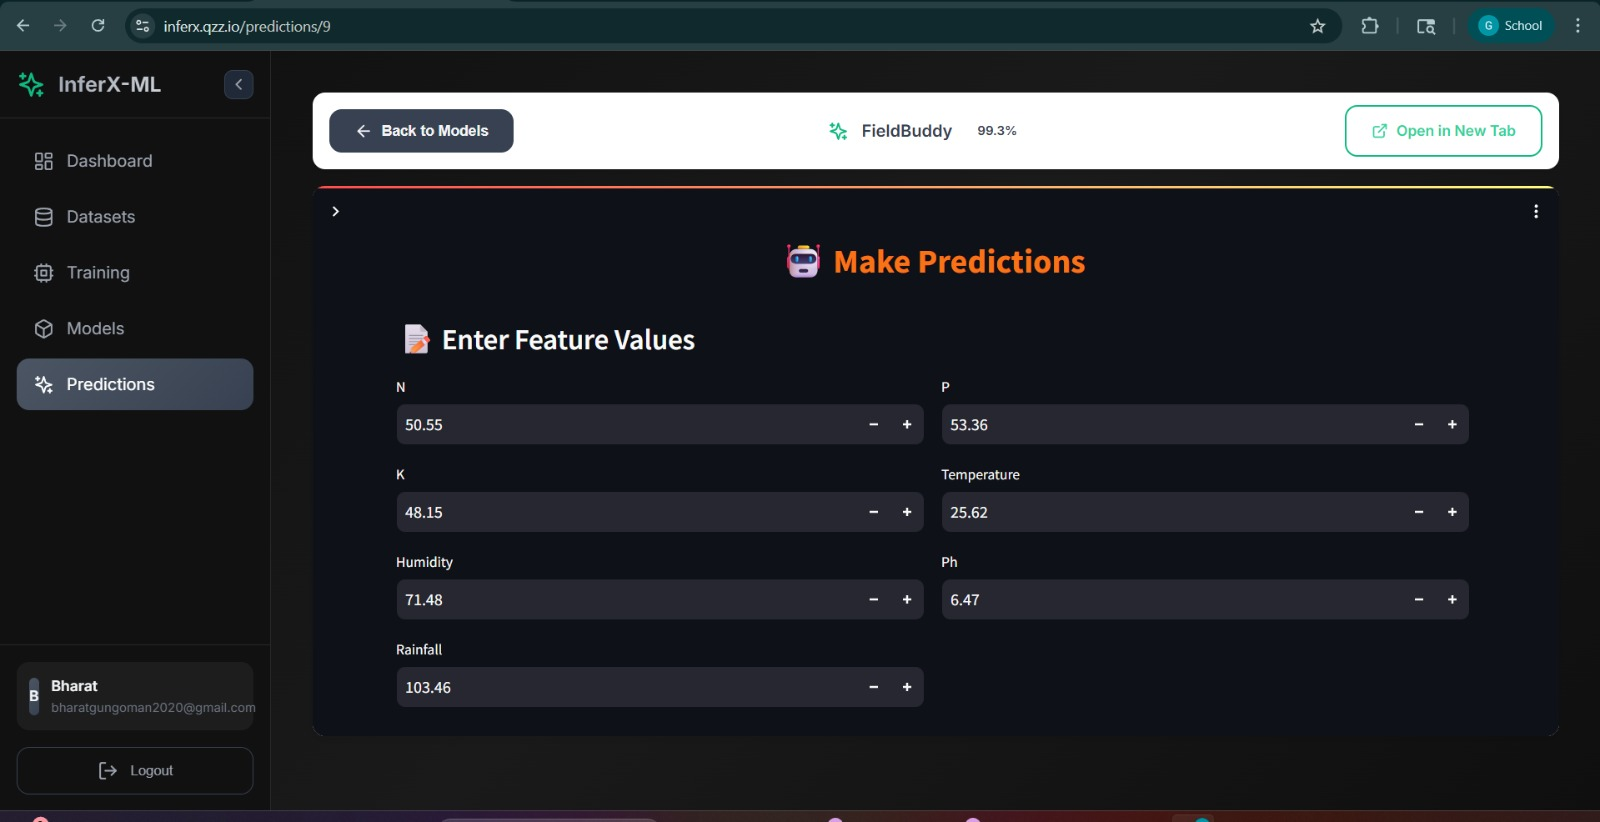
\includegraphics[width=1\textwidth]{images/10.jpeg}}
    \caption{Interface Page}
    \label{fig:img7}
\end{figure}

\begin{figure}[H]
    \centering
    \fbox{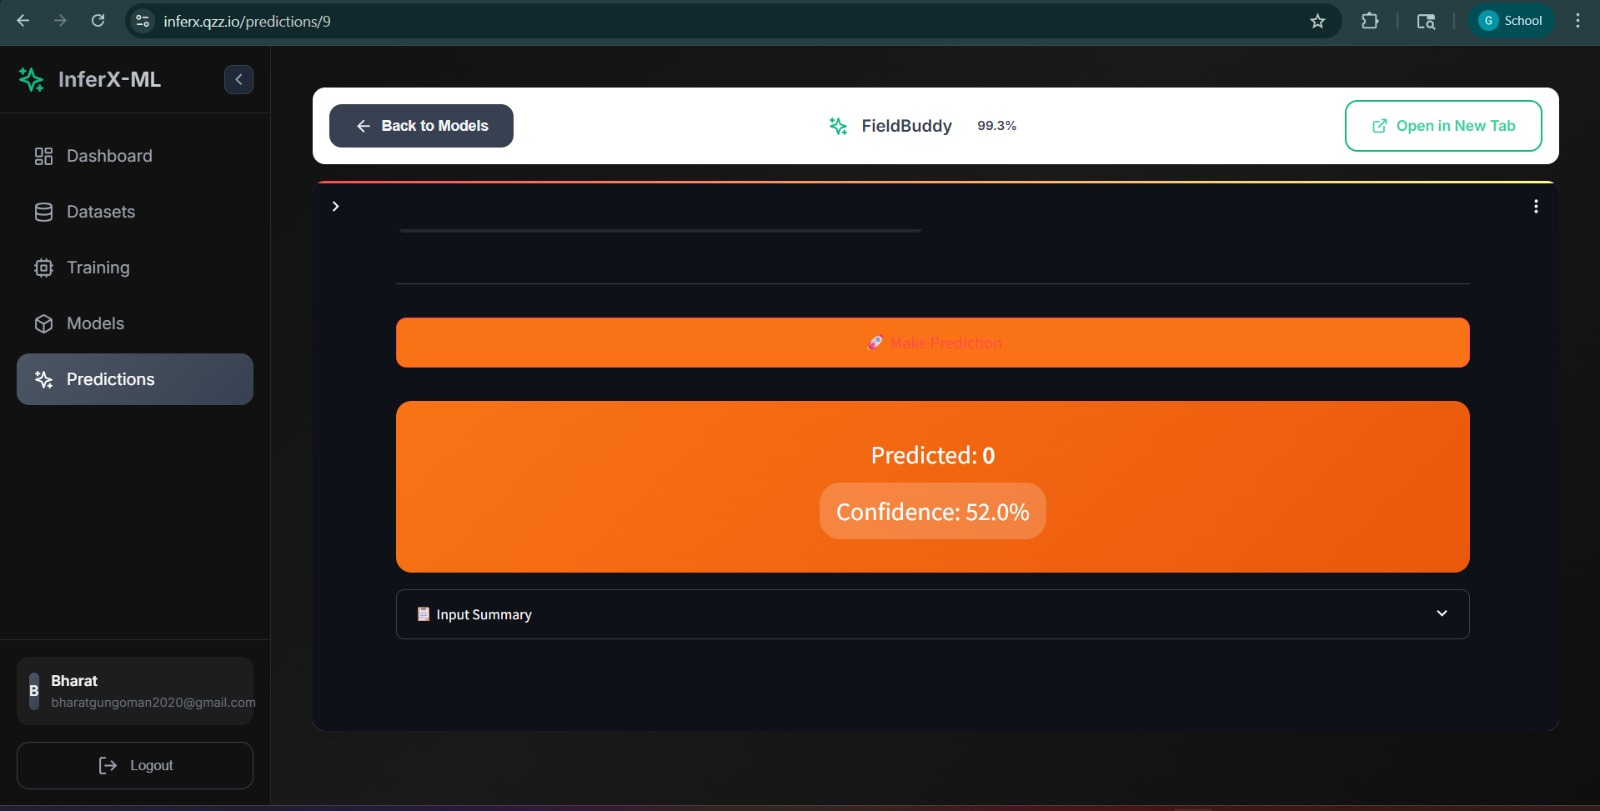
\includegraphics[width=1\textwidth]{images/11.jpeg}}
    \caption{Result Page}
    \label{fig:img7}
\end{figure}
\chapter{Conclusion}

\hspace{0.5cm}Machine learning holds immense potential for transforming decision-making across industries, yet its adoption remains severely limited by the technical expertise required to build, evaluate, and deploy predictive models. Traditional ML workflows demand proficiency in programming, data preprocessing, algorithm selection, and model interpretation, creating a significant barrier for domain experts, small businesses, educators, and students. Existing commercial AutoML platforms, while capable, are often expensive, proprietary, and function as black boxes that provide little transparency into how models are built or why specific predictions are made. These challenges result in a widening gap between the growing availability of data and the ability of non-technical users to extract meaningful insights from it.\vspace{0.3cm}

The proposed ``InferX ML'' platform directly addresses these challenges by providing a unified, no-code machine learning environment that automates the entire ML lifecycle, from data ingestion and intelligent profiling to model training, evaluation, and explainable predictions. It incorporates key capabilities such as rule-based AutoML across tabular, time-series, and image data, AI-powered natural language goal analysis via Google Gemini and Groq APIs, SHAP-based model explainability, and an auto-generated prediction user interface that sets it apart from existing tools in the market. Built on a modern, containerized microservices architecture using React, Flask, Streamlit, PostgreSQL, and MinIO, the platform is designed to be lightweight, scalable, and fully open-source. Ultimately, InferX ML serves as both a practical analytics tool and an educational incubator, empowering users to build production-ready models, understand AI-driven insights through transparent explanations, and gain hands-on experience with industry-standard ML workflows, thereby bridging the gap between raw data and intelligent, actionable predictions.\vspace{0.3cm}
\chapter{Future Scope}

\begin{itemize}

\item \textbf{Distributed Training Infrastructure:}

The platform can be enhanced with a distributed training system that allows users to leverage multiple servers and hardware resources such as CPUs and GPUs without requiring in-depth knowledge of cloud technologies. \\

\item \textbf{Continuous Model Retraining:}

To ensure that deployed models remain accurate and relevant over time, the platform will incorporate automated retraining mechanisms. \\
\item \textbf{Automated Hyperparameter Optimization:}

The platform can be extended to include advanced automated hyperparameter tuning techniques such as Bayesian Optimization and Genetic Algorithms. \\
\item \textbf{Real-Time Data Processing and Streaming Support:}

Future enhancements can introduce support for real-time data pipelines and streaming frameworks. \\

\item \textbf{Enhanced Model Explainability:}

Future improvements will focus on advancing model interpretability by integrating multiple explainability techniques such as SHAP and LIME. These tools will provide deeper insights into feature importance, local and global explanations, and decision boundaries of models. \\

\item \textbf{Cloud Deployment and API Integration:}

InferX ML will be extended to support seamless cloud deployment and API-based access to trained models. Users will be able to deploy models on cloud platforms and generate REST APIs for real-time inference. \\

\end{itemize}
\begin{thebibliography}{9}

\bibitem{hutter2019}
F. Hutter, L. Kotthoff, and J. Vanschoren, ``Automated Machine Learning: Methods, Systems, Challenges,'' Springer, 2019, doi: 10.1007/978-3-030-05318-5.

\bibitem{he2021}
X. He, K. Zhao, and X. Chu, ``AutoML: A Survey of the State-of-the-Art,'' \textit{Knowledge-Based Systems}, vol. 212, p. 106622, Jan. 2021, doi: 10.1016/j.knosys.2020.106622.

\bibitem{baratchi2024}
M. Baratchi et al., ``Automated Machine Learning: Past, Present and Future,'' \textit{Artificial Intelligence Review}, vol. 57, no. 122, 2024, doi: 10.1007/s10462-024-10726-1.

\bibitem{feurer2015}
M. Feurer et al., ``Efficient and Robust Automated Machine Learning,'' in \textit{Advances in Neural Information Processing Systems (NeurIPS)}, vol. 28, 2015.

\bibitem{olson2016}
R. S. Olson and J. H. Moore, ``TPOT: A Tree-Based Pipeline Optimization Tool for Automating Machine Learning,'' in \textit{Proc. AutoML Workshop, ICML, PMLR}, vol. 64, 2016.

\bibitem{zoller2021}
M.-A. Zöller and M. F. Huber, ``Benchmark and Survey of Automated Machine Learning Frameworks,'' \textit{Journal of Artificial Intelligence Research}, vol. 70, pp. 409–472, 2021, doi: 10.1613/jair.1.11854.

\bibitem{kreuzberger2022}
D. Kreuzberger, N. Kühl, and S. Hirschl, ``Machine Learning Operations (MLOps): Overview, Definition, and Architecture,'' \textit{arXiv preprint arXiv:2205.02302}, 2022, doi: 10.48550/arXiv.2205.02302.

\bibitem{gundersen2018}
O. E. Gundersen and S. Kjensmo, ``State of the Art: Reproducibility in Artificial Intelligence,'' \textit{AI Magazine}, vol. 39, no. 4, pp. 56–62, 2018, doi: 10.1609/aimag.v39i4.2815.

\bibitem{vanschoren2018}
J. Vanschoren, ``Meta-Learning: A Survey,'' \textit{arXiv preprint arXiv:1810.03548}, 2018, doi: 10.48550/arXiv.1810.03548.

\bibitem{lundberg2017}
S. M. Lundberg and S.-I. Lee, ``A Unified Approach to Interpreting Model Predictions,'' in \textit{Advances in Neural Information Processing Systems (NeurIPS)}, vol. 30, 2017.

\bibitem{xin2021}
D. Xin et al., ``Machine Learning in Production: A Review,'' \textit{ACM Computing Surveys}, vol. 54, no. 8, pp. 1--38, 2021.

\bibitem{waring2020}
J. Waring, C. Lindvall, and R. Umeton, ``Automated machine learning: Review of the state-of-the-art and opportunities for healthcare,'' \textit{Artificial Intelligence in Medicine}, vol. 104, p. 101822, 2020.

\bibitem{zoph2017}
B. Zoph and Q. V. Le, ``Neural Architecture Search with Reinforcement Learning,'' in \textit{International Conference on Learning Representations (ICLR)}, 2017.

\bibitem{kotthoff2017}
L. Kotthoff et al., ``Auto-WEKA 2.0: Automatic model selection and hyperparameter optimization in WEKA,'' \textit{Journal of Machine Learning Research}, vol. 18, no. 25, pp. 1--5, 2017.

\bibitem{paleyes2022}
A. Paleyes, R. G. Urma, and N. D. Lawrence, ``Challenges in Deploying Machine Learning: A Survey of Case Studies,'' \textit{ACM Computing Surveys}, vol. 55, no. 6, pp. 1--29, 2022.

\end{thebibliography}


\end{document}